\documentclass[conference,10pt]{IEEEtran}
%\documentclass[conference,draft,onecolumn]{IEEEtran}
% useful packages, copy and paste from diff sources

\usepackage[english]{babel}
\usepackage[T1]{fontenc}
\usepackage{cite,url,color} % Citation numbers being automatically sorted and properly "compressed/ranged".
\usepackage{graphics,amsfonts}
\usepackage{epstopdf}
\usepackage[pdftex]{graphicx}
\usepackage[cmex10]{amsmath}
% Also, note that the amsmath package sets \interdisplaylinepenalty to 10000
% thus preventing page breaks from occurring within multiline equations. Use:
\interdisplaylinepenalty=2500
% after loading amsmath to restore such page breaks as IEEEtran.cls normally does.
\usepackage[utf8]{inputenc}
% Useful for displaying quotations
%\usepackage{csquotes}
% Compact lists
%\let\labelindent\relax
\usepackage{enumitem}
\usepackage{multirow}
%tikz figures
\usepackage{tikz}
\usetikzlibrary{automata,positioning,chains,shapes,arrows}
\usepackage{pgfplots}
\usetikzlibrary{plotmarks}
\newlength\fheight
\newlength\fwidth
\pgfplotsset{compat=newest}
\pgfplotsset{plot coordinates/math parser=false}

\usepackage{array}
% http://www.ctan.org/tex-archive/macros/latex/required/tools/
%\usepackage{mdwmath}
%\usepackage{mdwtab}
%mdwtab.sty	-- A complete ground-up rewrite of LaTeX's `tabular' and  `array' environments.  Has lots of advantages over
%		   the standard version, and over the version in `array.sty'.
% *** SUBFIGURE PACKAGES ***
%\usepackage[tight,footnotesize]{subfigure}
\usepackage{subfig}

\usepackage[top=1.5cm, bottom=2cm, right=1.6cm,left=1.6cm]{geometry}
\usepackage{indentfirst}

\usepackage{times}
% make sections titles smaller to save space
%\usepackage{sectsty}
%\sectionfont{\large}
% enable the use of 'compactitem', a smaller 'itemize'
%\usepackage{paralist}

% MP
% to split equations using dmath env
\usepackage{breqn}
% nice rules in tables
\usepackage{booktabs}
\usepackage{lipsum}


%\setlength\parindent{0pt}
\linespread{1}

% MC
\newcommand{\MC}[1]{\textit{\color{red}MC says: #1}}
\newcommand{\AZ}[1]{\textit{\color{blue}AZ says: #1}}
\newcommand{\MP}[1]{\textit{\color{green}MP says: #1}}

\usepackage{placeins}


%%%%%%%%%%%%%%%%%%%%%%%%%%%%%%%%%%%%%%%%%%
\begin{document}
%%%%%%%%%%%%%%%%%%%%%%%%%%%%%%%%%%%%%%%%%%
\title{V2X mmWave Connectivity With Real Velocity Traces}

\author{\IEEEauthorblockN{Luca Della Libera, Andrea Rossi, Jacopo Pegoraro}
\IEEEauthorblockA{Department of Information Engineering, University of Padova -- Via Gradenigo, 6/b, 35131 Padova, Italy\\Email: {\tt\{luca.dellalibera.1, andrea.rossi.26, jacopo.pegoraro\}@studenti.unipd.it}
}}

\maketitle

\begin{abstract}
The mmWave band offers the opportunity to exceptionally increase the data rates for fifth-generation cellular systems and supports the birth of emerging automotive applications. The performance of end-to-end communicanications dramatically decreases when there are obstacles in the Line-Of-Sight (LOS) between a base station and an User Equipment (UE).
This paper analyzes the performance of UDP protocol under different handover policies, in a realistic urban automative scenario based on real-world traffic data simulation traces generated with SUMO (an open source simulator which allows traffic systems modelling) and imported in a network simulation platform such as ns-3. In a future urban scenario, important information such as the route of a car from a starting point to a destination could be effectively employed to predict which base station is more suitable to ensure a better connection. The purpose of this paper is showing that these policies, combined with prior knownledge of the scenario, can improve the throughput and/or delay of the connection.
\end{abstract}

%%%%%%%%%%%%%%%%%%%%%%%%%%%%%%%%%%%%%%%%%
\section{Introduction}\label{sec:intro}
%%%%%%%%%%%%%%%%%%%%%%%%%%%%%%%%%%%%%%%%%

In the last few years a vast number of automotive applications were developed and many of them are already being tested on the latest generation vehicles: self-driving cars, sensors for real time object recognition and infotainment are only some examples. However, a fundamental requirement to effectively implement these applications is to have high data rates communication capabilities, as the sensors and devices required could produce data in the order of magnitude of hundreds of Mb/s \cite{surveh}.
The state of the art protocol for communication in a vehicular environment is the \emph{dedicated short-range communication} (DSRC) that, however, cannot satisfy the mentioned requirements, having a theoretical rate of 27 Mb/s \cite{surveh}. For this reason, there is growing interest in the potential of mmWave technologies, that make use of the frequency spectrum over 10 GHz, providing data rates in the order of the Gb/s. These transmission capabilities can be achieved using carriers at very high frequency, therefore increasing the available bandwidth that could be exploited and consequently the capacity of the radio links. However, there are some drawbacks of this approach that become even more significant in outdoor and vehicular situations: one is the high attenuation that mmWave signals are subjected to, indeed the \emph{path-loss} in a radio channel depends on the reciprocal square-root of the wavelength $\lambda$, so reducing $\lambda$ (increasing frequency) the path-loss increases, thus there is need for more mmWave base stations (called also mmWave enhanced Node Base - eNB) to avoid lack of coverage. Another problem is that, in order to avoid the just mentioned high attenuation, massive MIMO is used to convey the signal into narrow directional beams instead of the isotropic transmission used in the present standards, so when facing a high speed nodes scenario as can be a vehicular one, mmWave technologies can perform poorly due to blockage and bad beam aligning \cite{mmvehicle}.

To partially solve these problems in a future urban scenario with high density of mmWave base stations, we can work on improving the handover (HO) procedure, that is the method used to control the switch of nodes between different base stations as they move in the scenario. The current handover procedure adopted in mmWave networks is the one inherited from the 4G-LTE standard and is based on connecting to the base station that provides the maximum received SINR among those that are reachable. In this paper, we simulated a typical urban scenario and we tested 4 different handover procedures, beginning with the standard one and then checking if slight modifications could lead to improvements in terms of throughput and/or delay.


%%%%%%%%%%%%%%%%%%%%%%%%%%%%%%%%%%%%%%%%%%%%
\section{Related Work}\label{sec:sota}
%%%%%%%%%%%%%%%%%%%%%%%%%%%%%%%%%%%%%%%%%%%%

The interest for mmWave band, between 30 and 300 GHz, where the available bandwidth is much wider than today's cellular networks, is growing more and more. Many researches have been conducted for analyzing challenges and opportunities that mmWave presents at different layers of the protocol stack, in order to support the massive demand for high data rates that is expected to be required in next generation of automotive applications.
Rangan et al. \cite{mmwpac} analyze various technologies including adaptive beamforming, multihop relaying, heterogeneous network architectures, and carrier aggregation used in the mmWave context, highlighting that these systems offer a capacity at least one order of magnitude higher than current state of the art LTE networks for what concerns outdoor coverage.

Regarding highly dense or highly mobile vehicular scenarios, Giordani et al. \cite{mmvehicle} observe that vehicles are subjected to frequent handover, and obstacles can undermine a successful communication even if the automotive nodes are perfectly aligned, since mmWave cannot penetrate through solid materials. Moreover, beam alignment can exploit known geographical position of the nodes in order to limit the search area of the most favorable beam direction. Anyway, according to their analysis, the performance of the automotive nodes strictly depends on parameters such as number and velocity of the nodes, beam tracking periodicity and specific environment in which the vehicles are deployed.

To better capture the most significant aspects of mmWave in vehicular networks, New York University and University of Padova developed an open-source mmWave module for ns-3, based on LTE architecture. Mezzavilla et al. \cite{e2esim} provide some interesting code examples, showing how this module can be used to set up a scenario.

Another interesting work, based on the improvement of the performance of a mmWave communication, has been proposed by Polese et al. \cite{imphand}, with the concept of Dual-Connectivity (DC): maintaining connections to multiple cells (both 5G mmWave cells and/or common 4G cells), users can find alternate routes to keep the connection.

None of the researches mentioned above analyzes what happens in a real-world scenario; for this reason this paper focuses on testing the results from previous works on a realistic urban traffic situation and developing new techniques, in order to achieve better performances in term of QoS metrics.

In the next sections we describe the simulation scenario and the handover policies, discussing the most relevant results of the simulation.


%%%%%%%%%%%%%%%%%%%%%%%%%%%%%%%%%%%%%%
\section{System Model}\label{sec:symo}
%%%%%%%%%%%%%%%%%%%%%%%%%%%%%%%%%%%%%%
The system model description is divided into two subsections. In the first one we describe the simulation scenario, pointing out which parameters can influence the simulation results and why we made certain choices to solve practical implementation problems.
In the second part, we present the different policies we tested to improve QoS metrics, focusing in particular on throughput and delay.

\subsection{Description of the simulation scenario}

\begin{figure*}[ht]
	\begin{center}    
		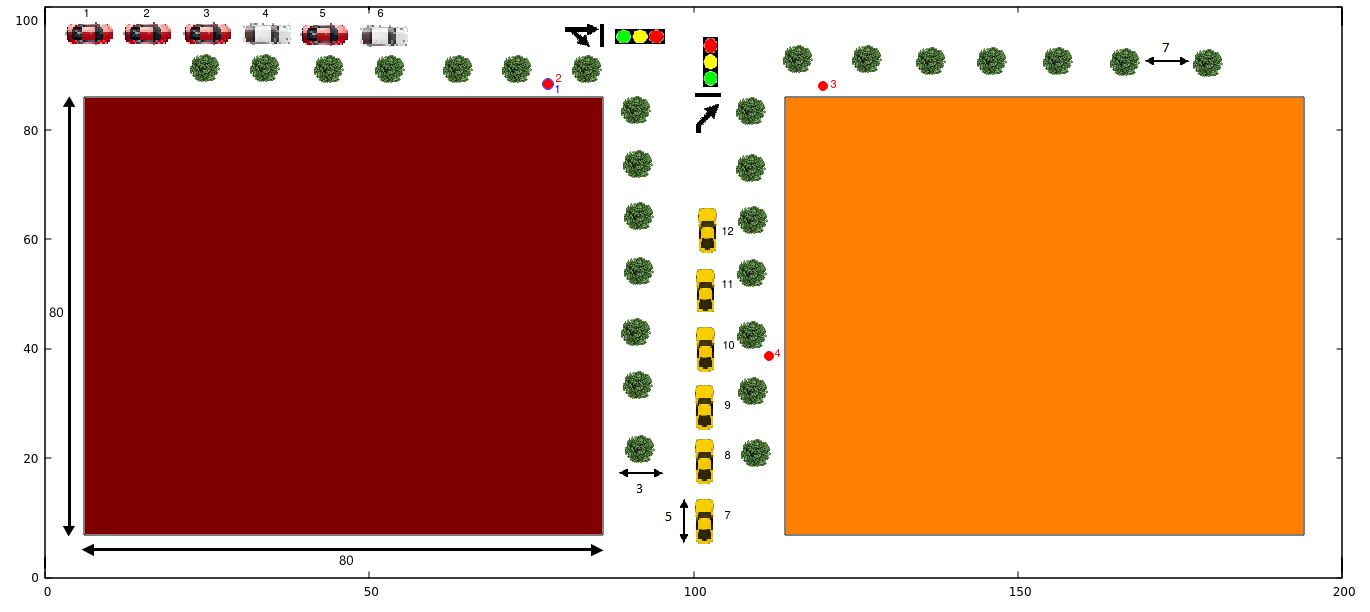
\includegraphics[width=14cm, keepaspectratio]{images/scenario3.png}
		\caption{The scenario, distances are expressed in [m].}
		\label{fig:scenario}
	\end{center}
\end{figure*}

\begin{table}[]
	\begin{center}
			\caption{Summary of the main simulation parameters.}
		\begin{tabular}{ccc}
			\toprule
			
		    Parameter & Value & Description  \\
			\midrule
			
			Sim. Time & 60 s & Total duration of the simulation \\
			Car speed & 0-13.8 m/s & Speed varies in this interval \\
			Pck. time & 1 $\mu$s & Application inter-packet required time \\
			Pck. dim. & 1054 byte & UDP packets dimension \\			
			T. light  & 45 s & Duration of the red traffic light \\ 			
			Min. dist. & 10 m & Min. distance between UEs and eNBs \\
			$D_{X2}$ & 500 $\mu$s & One-way delay on X2 links \\
			
			\bottomrule
		\end{tabular}
    \end{center}
	\label{tab:bay3}
\end{table}


The construction of the simulation scenario consists of two steps: the realization of the urban environment with SUMO, which generates realistic speed and position traces of the vehicles, and the usage of these traces to build the network infrastructure with ns-3.
For what concerns the first step, we decided to keep the environment as simple as possible, without sacrificing a minimum amount of complexity that is required to make the mmWave connectivity as challenging as it could be in a real urban vehicular environment. For this reason, we reproduced a T-shaped crossroad with a traffic light in the middle (Figure 1). The horizontal road has only one lane, while the vertical one has two, allowing traffic in both directions. There are 12 cars divided into 3 flows, depending on the path they follow: UEs 1, 2, 3, 5 belong to the left-to-right flow, UEs 4 and 6 to the left-to-bottom flow, UEs 7, 8, 9, 10, 11, 12 to the bottom-to-right flow.
At first, the traffic light is green for the bottom-to-right flow and for the left-to-bottom flow, therefore UEs 6, 7, 8, 9, 10, 11, 12 are allowed to go (notice that UE 4 cannot move even though it belongs to the left-to-bottom flow, because there is only one lane and a car is on its way). After 45 s, the traffic light switches and all the UEs reach their destinations.


Regarding the second step, the mobility traces of the vehicles were imported in ns-3, and using mmWave module developed by University of Padova and New York University, we deployed 3 base stations, in particular 2 pure mmWave eNBs (eNB 3, 4 in Figure 1) and one hybrid mmWave-LTE eNB, that acts as a link towards the Internet and allows to use the DC mechanism previously mentioned, in order to achieve a more reliable connection. Furthermore, it serves as a coordinator for the handover procedures, in the sense that it decides, according to some criterion, after collecting information on the other eNB SINRs , which UE connects to which eNB. In our implementation, the hybrid eNB consists of two overlapping eNBs (eNB 1, 2 in Figure 1), a mmWave and a LTE one, which are deployed in the same position. To make the scenario more realistic, buildings and trees were added at the sides of the roads to prevent UEs from being always in LOS condition, making connection harder to establish. The physical details of the scenario are shown in Figure 1.


The networking side of the model was realized using \texttt{MmWaveHelper} class of mmWave ns-3 module, which installs the mmWave physical channel and the upper layers of the protocol stack in all the devices involved in the simulations (included the X2 protocol for the communication between the LTE station and the other eNBs). In our case, it consists of IP addressing and UDP configuration. The core network, which provides Internet connectivity to all the nodes, was simulated through a gateway connected to the LTE eNB and a remote host, connected to the gateway. 

The channel model adopted in this scenario is 3GPP-UmiStreetCanyon, which is reliable provided that 2D distance between eNB and UE is always greater than 10 m. The maximum bitrate that can be achieved with this configuration is 3 Gb/s for each eNB. In a real-world scenario, problems occur when the total throughput required by UEs exceeds eNBs capacity. In order to saturate the eNBs, we ran on each UE a UDP application which demands about 8 Gb/s of traffic for the whole time the node is connected.

This scenario was used to test four different handover procedures, which will be presented in the next section.



\noindent
\subsection{Handover policies}
The following four policies were tested on the simulation scenario:


\begin{enumerate}
\item DHO: Default HandOver is the standard rule used nowadays by LTE cellular networks and has its core in the criterion used by the LTE coordinator to decide when a UE has to switch between two base stations. The procedure is summarized in the following steps \cite{imphand}:

\begin{itemize}
	\item The coordinator monitors the received SINR by an UE from all the eNBs.
	\item Whenever a eNB (target cell) provides a SINR at least 3 dB higher than the current one, the coordinator keeps track of the difference between the two SINRs for a time equal to TTT (Time-To-Trigger) seconds.
	\item If the new eNB keeps providing more than 3 dB better SINR for all the duration of TTT, the coordinator makes the UE switch to the new eNB.
\end{itemize}

In \cite{imphand}, the authors analyze two different ways to choose the TTT value: one is to keep it fixed at, for example, $f_{TTT}=150ms$, and the other is to have a \emph{dynamic} threshold that is higher if the difference $\Delta$ between the current eNB SINR and the target is smaller. 

\item MHO100:
Modified HandOver 100 relies on a threshold value for SINR, that we will call SINR*:

\begin{itemize}
	\item The coordinator keeps track of the maximum SINR received for each UE.
	\item If there are SINRs from one or more eNBs that are close to the maximum one, in the sense that the difference between the two is lower than SINR*, the coordinator triggers the handover towards the eNB that has the lowest number of UEs connected.
	\item If, according to the previous rule, none of the eNB is a good candidate for handover, UE connects to the maximum SINR eNB.
	If there are many candidate eNB with the same number of connected UEs, the one with higher SINR is preferred.
\end{itemize}

The goal of this method is considering that throughput and delay may strongly depend on the level of congestion of the eNBs, due to the excessive number of vehicles connected. SINR is indeed a good metric of path-loss, blockage and quality of the channel, but it does not include the number of resources the eNB is currently handling.

\item MHOM:
Modified HandOver Mean follows the same procedures of MHO100, with a different threshold value, computed as the average of the SINRs received from the 3 mmWave eNBs. In this way, SINR* is able to adapt to different circumstances, considering the fact that in such a dynamic scenario, SINR usually varies exponentially from 1 dB up to 40-60 dB. Furthermore, since SINR* is a function of the SINR of all eNBs, it can handle situations in which the 3 SINRs are very different from one another.



\item MHOS:
Modified HandOver Shannon is based on a different approach. The goal is maximizing the capacity of the channel used by the UEs, taking into account the congestion by means of Shannon formula for channel capacity. Indeed, the channel capacity offered by a base station $i$ can be approximately expressed as:
 $$
 C_i=\frac{1}{N_i} B \log(1+SINR_i)
 $$
\noindent where $N_i$ is the number of UEs connected to the $i$-th eNB, $B$ is the channel bandwidth and $SINR_i$ is the received SINR from the base station $i$.
The proposed policy is the following:

\begin{itemize}
	\item The UE is initially connected to the eNB $i$.
	\item The coordinator triggers the handover towards the eNB $j$ if the channel capacity offered by the target base station is higher than the current one. In formulas:
	$$
	\frac{1}{N_i} \log(1+SINR_i) < \frac{1}{N_j+1} \log(1+SINR_j)
	$$ 
\end{itemize}
\noindent Notice that the bandwidth can be simplified from the expression and that $N_j$ has to be incremented by one since, if the handover is performed, the target eNB will have one more UE to handle.
\end{enumerate}

It is worth noticing that the 3 modified policies take into account, even though in an indirect way, the route followed by a UE, because at every instant the number of UEs connected to a certain eNB depends on how the scenario has evolved in the past. For instance, the UEs enqueued at the traffic light, will try to connect to the closest eNB. With DHO policy, as the vehicles continue to arrive, the eNB will rapidly reach a situation of congestion. With a MHO policy instead, there are good chances that UEs closer to the crossroad, receiving a lower but still good signal from another eNB, which is not saturated (because the cars coming from the other road are moving, since the traffic light is green for them), will switch to this eNB, freeing up resources for the other UEs. In such a situation, MHO policy is able to indirectly 'detect' the presence of a traffic light, and act consequently. These policies are indeed a mixture between the current memoryless policies, and the smart policies of the future, which will be developed when self driving vehicles, able to communicate their information to the eNBs in real time, will become reality.



\begin{figure*}[h] \label{fig:4pol}
	\begin{center}
		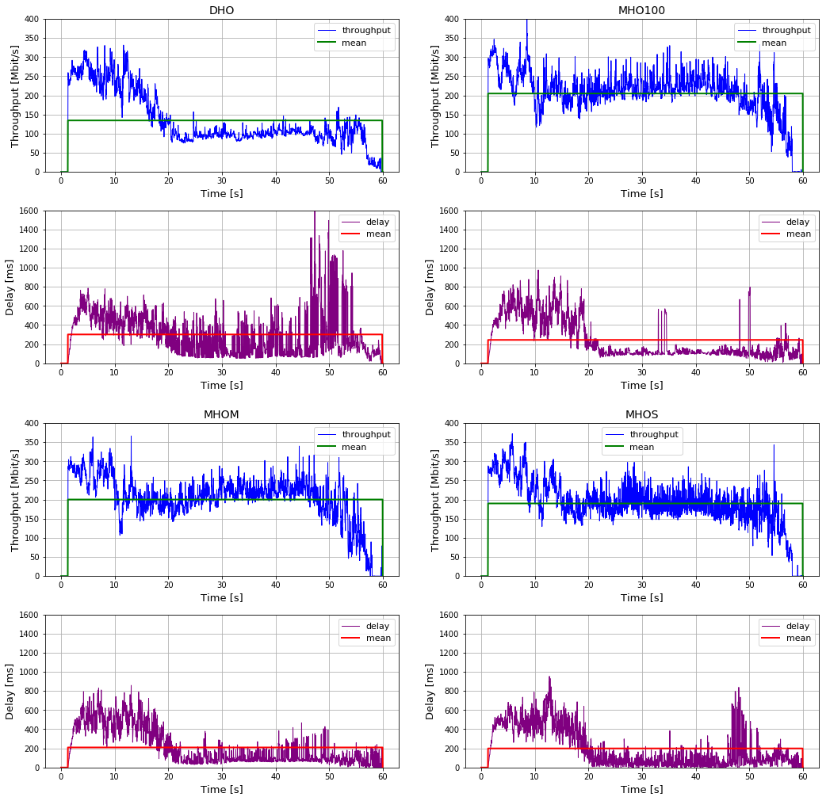
\includegraphics[scale=0.85]{images/confronto.png}
		\caption{Comparison among 4 handover policies}
	\end{center}
\end{figure*}


%%%%%%%%%%%%%%%%%%%%%%%%%%%%%%%%%%%%%%%%%%%%%%%
\section{Results}\label{sec:res}
%%%%%%%%%%%%%%%%%%%%%%%%%%%%%%%%%%%%%%%%%%%%%%%

In this section, we explain the mathematical approach we used to analyze data and we compare DHO with the other three policies described above.
Since the scenario is deterministically defined, we decided to include some kind of randomness in the channel, for extending the validity of the analysis to more general urban traffic situations. Therefore, we ran 5 simulations per policy, initializing ns-3 random number generator with different seeds, and we computed the instantaneous throughput and delay of each UE as mean of the data collected in the 5 simulations. The throughput has been computed on downlink at PDCP layer, sampling the received packets trace every 5 ms, summing the total amount of bits received in this interval and dividing by its duration, as described in \cite{imphand}. 
The small number of run simulations is due to the high computing power needed to simulate such transmission rate, typical of mmWave system. However, we noticed that, how it was expected to be, the results were not uniform for all UEs: some of them experienced a high improvement of throughput and delay, while the other a worsening of the same. In order to evaluate the global performance of the policy, we computed mean instantaneous throughput and delay over the 12 UEs, and then calculated the corresponding time average value.
Figure 2 shows the final results of the 4 policies. The plot show a decreasing trend towards the end of the simulation which is caused by the variable number of UE in the scenario, since UE which have crossed the intersection are considered disconnected from the network.

Each proposed method reaches an improvement of about 25\% for the mean throughput, while regarding the delay, its mean reaches a decrease of about 30\%. Among the proposed policies, MHOM can be considered the best respect to throughput because even if MHO100 reaches the best mean throughput, it is less flexible because the threshold is fixed and it maybe it would not perform equally good in a different scenario . Regarding the delay, MHOS offers the least mean delay among the policies but if we have to decide the more suitable it is needed a trade off between these two metrics. In all the simulations, however, we noticed the strong impact of the urban scenario on the performances of the policies. In many cases the UEs experience blockage and a consequent drop in the instantaneous throughput due to the many obstacles present, causing the highly oscillating behavior of both throughput and delay that can be seen in the plots.

An interesting fact that is evident from the plots is that the proposed methods improve the throughput and delay especially in the part of the simulation that starts at about 15-20 s. That is the moment when the first flow of cars, coming from the bottom road exit the simulation and the second flow is stopped by the traffic light. This is exactly what was expected: in our methods we tried to improve the way in which the handover procedures handles the congestion of a eNB, so when there is a moment in which 6 cars are not moving the standard procedure makes them connect all to the nearest base station, while our policies tend to split the group among two eNBs.

Another result that has to be compared among this different methods is the number of handover events that occur during the simulation. Table II briefly summarizes from a numerical point of view the number of these events, mean throughput and mean delay. The proposed techniques need a bigger number of switches between eNBs in order to improve the end-to-end communication with respect to the analyzed metrics and this could be a problem if this number becomes too high because the handover procedure takes time and has a little but non indifferent impact on the overall delay. For this reason MHOM proves to be the best trade-off between performance improvement and number of switches among all the policies.

\begin{table}[]
\centering
\caption{Comparison table of the handover policies}
\label{my-label}
\begin{center}
	
\begin{tabular}{cccc}
	\toprule

\multirow{3}{1.8cm}{Handover policy} & \multirow{3}{2cm} {Mean throughput [Mbit/s]} & \multirow{3}{1.8cm} {Mean delay [$\mu$s]} &\multirow{3}{1.8cm}{Mean number of ho events}  \\ 
 &  &  &   \\
 &  &  &   \\ 
 \midrule

DHO    & 134.55          & 301.96          & \textbf{190.0} \\ 
MHO100 & \textbf{204.89} & 244.74          & 218.2          \\
MHOM   & 200.07          & 209.7           & 203.6          \\ 
MHOS   & 189.81          & \textbf{199.44} & 249.2          \\ 

\bottomrule
\end{tabular}
\end{center}
\end{table}


%%%%%%%%%%%%%%%%%%%%%%%%%%%%%%%%%%%
\section{Conclusions}\label{sec:conclusion}
%%%%%%%%%%%%%%%%%%%%%%%%%%%%%%%%%%%

In realistic urban automotive scenario the number of UE connected to the more suitable eNB could be large, creating congestion problem especially in same local areas like crossroads, traffic roundabouts or level crossings. In this paper we proposed three different handover policies in order to improve the mean throughput and to decrease the mean delay of the UEs.

 Performing some simulations on a simple but realistic urban environment we noticed the following things:
\begin{itemize}
\item The proposed handover policies are able to improve the performance of an end-to-end network with mmWave access links with respect to throughput and delay up to 25\% and 30\% respectively.
\item MHO100, with a fixed SINR threshold, has proved to obtain the best results in terms of throughput.
\item MHOS, based on the Shannon capacity, obtains the least delay.
\item MHOM is however the best trade-off between the two metrics, also because of its better adaptability to other scenarios and the relatively low number of handover events it triggers.
\end{itemize}

Also, regardless of the particular method considered, we proved that the standard handover procedure can be improved significantly by taking into account the number of UEs connected to each eNB. This approach can be considered as a first step towards a handover procedure that is based on the path followed by each vehicle, assuming that in the near future this kind of information will be more and more accessible due to the sharing of GPS tracks in real time in a self-driving cars context. 

Possible future developments of this work can be on one hand the modification of the scenario, creating some level of randomness in the positions and density of the obstacles and eNBs and also increasing the complexity reproducing situations with more cars or different kind of roads. It woud be also interesting to simulate the presence of pedestrians that can randomly cause blockage on the eNBs. 
On the other hand we aim to come up with possibly better solutions to improve even more the QoS metrics, maybe including some level of prediction on the movements of the vehicles based on both the knowledge of the map of the roads and the path followed by each car.



\addtocontents{toc}{Bibliografia}
\begin{thebibliography}{15}
	
	\bibitem{surveh}
	V. Va, T. Shimizu, G. Bansal, R. W. Wealth Jr et al.,
	\textit{Millimiter Wave vehicular communications: a survey}. 
	Foundations and trends in Networking, vol. 10, no. 1, 2016..
	
	\bibitem{mmvehicle}
	M. Giordani, A. Zanella, M. Zorzi,
	\textit{Millimiter Wave Communication in Vehicuar Networks: Challenges and Opportunities}. 
	IEEE 6th International Conference on Modern Circuits and System Technologies, 2017.
	
	\bibitem{imphand}
	M. Polese, M. Giordani, M. Mezzavilla, S. Rangan, M. Zorzi,
	\textit{Improved Handover Through Dual Connectivity in 5G mmWave Mobile Networks}. 
	IEEE Journal on Selected Areas in Communications, vol. 35, no. 9, pp. 2069-2084, 2017.
	
	\bibitem{e2esim}
	M. Mezzavilla, M. Zhang, M. Polese, R. Ford, S. Dutta, S. Rangan, M. Zorzi,
	\textit{End-to-End Simulation of 5G mmWave Networks}. 
	arXiv preprint, 2017.
	
	\bibitem{mmwwicom}
	T. S. Rapparport, R. W: Heath Jr, R. C. Daniels, J.N. Murdock,
	\textit{Millimeter Wave Wireless communications}.
	Prentice Hall, 2015.
	
	\bibitem{mmwcomsy}
	K. C. Huang, P. Rapajic, Z. Wang
	\textit{Millimiter Wave Communication Systems}.
	Wiley, 2011.
	
	\bibitem{mmwpac}
	S. Rangan, T. S. Rappaport, E. Erkip,
	\textit{Millimiter-Wave Cellular Wireless Netwoeks: Potentials and Challenges}
	Proceedings of the IEEE, vol. 102, no. 3, March 2014
	
\end{thebibliography}

\end{document}
